% IEEE Journal Paper
% Performance Evaluation of Event-Driven Banking Microservices
% Using Apache Kafka and Spring Boot Under High-Concurrency Workloads
%
% Author: Ayshi Shannidhya Panda
% Institution: Silicon Institute of Technology, Sambalpur, Odisha, India
% Department: Department of Computer Science and Engineering
%
% IMPORTANT: This manuscript uses the IEEEtran document class.
% Download IEEEtran.cls from: https://www.ieee.org/conferences/publishing/templates.html
% or install via your TeX distribution (e.g., texlive-publishers on Linux).

\documentclass[journal]{IEEEtran}

% ========================
% PACKAGES
% ========================
\usepackage[utf8]{inputenc}
\usepackage[T1]{fontenc}
\usepackage{amsmath,amssymb,amsfonts}
\usepackage{algorithmic}
\usepackage{algorithm}
\usepackage{graphicx}
\usepackage{textcomp}
\usepackage{xcolor}
\usepackage{booktabs}
\usepackage{multirow}
\usepackage{tabularx}
\usepackage{url}
\usepackage{hyperref}
\usepackage{cite}
\usepackage{balance}
\usepackage{listings}
\usepackage{tikz}
\usepackage{pgfplots}
\usepackage{pgfplotstable}
\usepackage{subcaption}
\usepackage{siunitx}
\usepackage{float}

\pgfplotsset{compat=1.18}
\usetikzlibrary{shapes.geometric, arrows.meta, positioning, calc, fit, backgrounds}

% ========================
% LISTING STYLE
% ========================
\definecolor{codegreen}{rgb}{0,0.6,0}
\definecolor{codegray}{rgb}{0.5,0.5,0.5}
\definecolor{codepurple}{rgb}{0.58,0,0.82}
\definecolor{backcolour}{rgb}{0.97,0.97,0.97}

\lstdefinestyle{javastyle}{
    backgroundcolor=\color{backcolour},
    commentstyle=\color{codegreen},
    keywordstyle=\color{blue}\bfseries,
    numberstyle=\tiny\color{codegray},
    stringstyle=\color{codepurple},
    basicstyle=\ttfamily\scriptsize,
    breaklines=true,
    frame=single,
    numbers=left,
    numbersep=5pt,
    showstringspaces=false,
    tabsize=2,
    captionpos=b
}

\lstdefinestyle{yamlstyle}{
    backgroundcolor=\color{backcolour},
    basicstyle=\ttfamily\scriptsize,
    breaklines=true,
    frame=single,
    captionpos=b
}

% ========================
% METADATA
% ========================
\hypersetup{
    colorlinks=true,
    linkcolor=blue,
    citecolor=blue,
    urlcolor=blue,
    pdftitle={Performance Evaluation of Event-Driven Banking Microservices Using Apache Kafka and Spring Boot Under High-Concurrency Workloads},
    pdfauthor={Ayshi Shannidhya Panda}
}

\begin{document}

% ========================
% TITLE
% ========================
\title{Performance Evaluation of Event-Driven Banking Microservices Using Apache Kafka and Spring Boot Under High-Concurrency Workloads}

\author{
    \IEEEauthorblockN{Ayshi Shannidhya Panda}
    \IEEEauthorblockA{
        Department of Computer Science and Engineering\\
        Silicon Institute of Technology\\
        Sambalpur, Odisha, India\\
        asp45624@gmail.com
    }
}

\maketitle

% ========================
% ABSTRACT
% ========================
\begin{abstract}
Microservice architectures have become the standard for building scalable financial applications, yet the choice of inter-service communication paradigm---synchronous REST, message-oriented middleware (RabbitMQ), or distributed event streaming (Apache Kafka)---remains insufficiently characterized under realistic banking workloads. This paper presents a systematic empirical evaluation of three communication strategies implemented within \textit{Neptune Bank}, a cloud-native banking platform comprising eight microservices built with Spring Boot~3.5 and Java~21, deployed via Docker on PostgreSQL databases. We design and execute controlled experiments using Apache JMeter and Gatling under graduated concurrency levels (100 to 20,000 concurrent users), measuring throughput, end-to-end latency (p50, p95, p99), CPU and memory utilization, Kafka consumer lag, error rate, and mean time to recovery (MTTR). A communication strategy abstraction layer enables switching between REST, RabbitMQ, and Kafka via Spring Profiles without modifying business logic. We apply Little's Law, Amdahl's Law, and queueing-theoretic models to interpret the observed scaling behavior. Fault tolerance experiments simulate broker crashes, service failures, and database slowdowns using chaos engineering techniques. Statistical analysis using ANOVA, confidence intervals, and hypothesis testing validates the significance of observed differences. Results demonstrate that Kafka-based event-driven communication achieves [TO BE FILLED AFTER EXPERIMENTS] improvement in throughput and [TO BE FILLED] reduction in p99 latency compared to synchronous REST under high-concurrency workloads, while RabbitMQ occupies an intermediate position. We identify the concurrency crossover point at which event-driven architecture outperforms synchronous communication and discuss the architectural trade-offs between consistency, latency, throughput, operational complexity, and fault tolerance. All source code, benchmarking scripts, Docker configurations, and raw experimental data are publicly available for reproducibility.
\end{abstract}

\begin{IEEEkeywords}
Microservices, Apache Kafka, Spring Boot, Event-Driven Architecture, Performance Evaluation, Distributed Systems, Banking Systems, Message Queuing, RabbitMQ, High Concurrency, Cloud-Native Architecture, Fault Tolerance
\end{IEEEkeywords}

% ========================
% I. INTRODUCTION
% ========================
\section{Introduction}
\label{sec:introduction}

\IEEEPARstart{T}{he} financial services industry has undergone a fundamental architectural transformation over the past decade, migrating from monolithic enterprise applications toward microservice-based architectures that promise improved scalability, independent deployability, and technology heterogeneity~\cite{newman2015building, dragoni2017microservices}. Modern banking platforms must simultaneously satisfy stringent requirements: sub-second transaction processing, 99.99\% availability, regulatory compliance for audit trails, and the ability to handle traffic spikes that can exceed 10$\times$ normal volumes during events such as month-end salary deposits, festive-season sales, or flash promotions~\cite{cockcroft2016netflix}.

A critical design decision in any microservice architecture is the choice of inter-service communication paradigm. Synchronous communication via REST APIs provides simplicity, immediate consistency, and straightforward debugging, but introduces tight temporal coupling between services---if a downstream service is slow or unavailable, the upstream caller blocks or fails~\cite{richardson2018microservices}. Asynchronous messaging through brokers such as RabbitMQ provides temporal decoupling with reliable message delivery guarantees, but introduces operational complexity and eventual consistency semantics~\cite{videla2012rabbitmq}. Distributed event streaming platforms such as Apache Kafka~\cite{kreps2011kafka} offer a third paradigm: durable, partitioned, append-only commit logs that enable both publish-subscribe messaging and event sourcing, with high throughput and horizontal scalability, but at the cost of increased infrastructure complexity and the challenges of exactly-once processing semantics.

Despite the proliferation of microservice adoption in the banking sector, the existing literature lacks systematic empirical comparisons of these three communication paradigms within a single, realistic banking application under controlled, statistically rigorous experimental conditions. Prior studies have predominantly focused on binary comparisons (REST vs.\ a single messaging technology), used synthetic or oversimplified workloads, or reported results without adequate statistical analysis~\cite{villamizar2015infrastructure, al2016comparison}. Furthermore, few studies provide open-source implementations and raw experimental data, limiting reproducibility.

\subsection{Research Gap}
\label{subsec:research_gap}

Our analysis of the existing literature reveals the following unresolved gaps:

\begin{enumerate}
    \item \textbf{Lack of three-way comparison}: Most studies compare two communication paradigms. A systematic comparison of REST, RabbitMQ, and Kafka within an identical application under identical workloads has not been adequately addressed.
    \item \textbf{Unrealistic workloads}: Many benchmarks use trivially simple operations (e.g., key-value lookups) that do not reflect the transactional complexity of banking operations involving cross-service coordination, database writes, and compensating transactions.
    \item \textbf{Absence of fault tolerance analysis}: Performance is typically measured only under normal conditions. The behavior of each communication paradigm under broker failure, service crash, and degraded network conditions is rarely quantified.
    \item \textbf{Missing statistical rigor}: Results are often reported as single-run averages without confidence intervals, statistical tests, or discussion of threats to validity.
    \item \textbf{Reproducibility deficit}: Source code, deployment configurations, and raw data are rarely made publicly available.
\end{enumerate}

\subsection{Contributions}
\label{subsec:contributions}

This paper makes the following contributions:

\begin{enumerate}
    \item We design and implement a complete cloud-native banking platform (\textit{Neptune Bank}) with eight microservices, featuring a novel \textit{communication strategy abstraction layer} that enables runtime switching between REST, RabbitMQ, and Kafka via Spring Profiles.
    \item We conduct a systematic three-way empirical comparison under graduated concurrency levels (100 to 20,000 users) across seven banking scenarios, measuring throughput, latency distribution, resource utilization, and error rates.
    \item We perform controlled fault tolerance experiments using chaos engineering techniques and quantify Mean Time to Recovery (MTTR), message loss rate, and data consistency under failure conditions.
    \item We apply queueing-theoretic models (Little's Law, Amdahl's Law, M/M/c queue models) to explain the observed scaling behavior and identify the concurrency crossover point.
    \item We provide all source code, Docker configurations, benchmarking scripts, and raw experimental data as an open-source repository for full reproducibility.
\end{enumerate}

\subsection{Paper Organization}
\label{subsec:organization}

The remainder of this paper is organized as follows. Section~\ref{sec:related_work} reviews related work and identifies the research gap. Section~\ref{sec:architecture} describes the system architecture. Section~\ref{sec:methodology} presents the experimental methodology. Section~\ref{sec:experimental_setup} details the experimental setup. Section~\ref{sec:results} presents the experimental results. Section~\ref{sec:discussion} discusses the findings and trade-offs. Section~\ref{sec:threats} identifies threats to validity. Section~\ref{sec:future_work} outlines future work. Section~\ref{sec:conclusion} concludes the paper.


% ========================
% II. RELATED WORK
% ========================
\section{Related Work}
\label{sec:related_work}

This section surveys the existing literature on microservice communication paradigms, event-driven architectures, and performance evaluation of distributed banking systems. We organize the review into four thematic areas.

\subsection{Microservice Architecture and Communication Patterns}
\label{subsec:rw_microservices}

The microservice architectural style, formalized by Newman~\cite{newman2015building} and Fowler and Lewis~\cite{fowler2014microservices}, decomposes applications into independently deployable services communicating over lightweight protocols. Richardson~\cite{richardson2018microservices} classifies inter-service communication into synchronous (request/response) and asynchronous (messaging) patterns, noting that synchronous communication creates temporal coupling that can cascade failures across service boundaries.

Dragoni et al.~\cite{dragoni2017microservices} provide a comprehensive survey of microservice challenges, identifying inter-service communication as a critical design decision that affects scalability, reliability, and consistency. Alshuqayran et al.~\cite{alshuqayran2016systematic} conducted a systematic mapping study of 33 primary studies and found that REST was the dominant communication mechanism, with limited empirical evidence on the performance implications of alternative approaches.

Villamizar et al.~\cite{villamizar2015infrastructure} compared monolithic and microservice deployments on AWS, reporting that microservices achieved comparable response times but required more infrastructure. However, their study did not compare different inter-service communication paradigms within the microservice architecture itself.

\subsection{Event-Driven Architecture and Apache Kafka}
\label{subsec:rw_kafka}

Event-driven architecture (EDA) has emerged as a paradigm for building loosely coupled, scalable systems~\cite{michelson2006event}. Kafka, originally developed at LinkedIn~\cite{kreps2011kafka}, has become the de facto standard for distributed event streaming, processing trillions of messages daily at organizations including LinkedIn, Netflix, and Uber~\cite{kafka_documentation}.

Dobbelaere and Esmaili~\cite{dobbelaere2017kafka} conducted a comparative study of Kafka and RabbitMQ, finding that Kafka achieved up to 15$\times$ higher throughput for simple message passing, while RabbitMQ provided lower latency for small message sizes and more flexible routing. However, their benchmarks used standalone producers and consumers without the overhead of an application framework.

Thein et al.~\cite{thein2014apache} analyzed Kafka's performance under varying partition counts and replication factors, reporting near-linear throughput scaling with partitions up to the number of available CPU cores. Wang et al.~\cite{wang2015building} explored Kafka in real-time data pipeline architectures, demonstrating sustained throughput of over one million messages per second.

Le Noac'h et al.~\cite{lenoach2017performance} benchmarked multiple message brokers (Kafka, RabbitMQ, ActiveMQ, NATS) across varying message sizes and consumer counts, finding that Kafka's throughput advantage increased with message size due to its sequential disk I/O model.

\subsection{Performance Evaluation of Microservice Systems}
\label{subsec:rw_performance}

Empirical performance evaluation of microservice systems has received increasing attention. Al-Debagy and Martinek~\cite{al2016comparison} compared REST and gRPC for microservice communication, finding that gRPC reduced latency by 30--50\% for small payloads due to HTTP/2 multiplexing and Protocol Buffers serialization.

Ueda et al.~\cite{ueda2016workload} proposed a workload characterization methodology for cloud applications, emphasizing the importance of representative traffic patterns and multi-metric analysis rather than single-dimensional throughput measurements.

Gan et al.~\cite{gan2019open} introduced DeathStarBench, an open-source benchmark suite for microservices, demonstrating that end-to-end latency is dominated by queuing delays at high utilization levels, consistent with queueing-theoretic predictions. Their methodology of using statistically rigorous experimental design with multiple runs and confidence intervals has influenced our approach.

Sriraman and Wenisch~\cite{sriraman2018mutune} investigated microservice tail latency, showing that 99th-percentile latency can be 10$\times$ the median, and that resource contention between co-located services significantly affects tail latency.

\subsection{Banking and Financial System Architecture}
\label{subsec:rw_banking}

Banking systems present unique challenges for microservice architectures due to ACID transaction requirements, regulatory compliance, and extreme reliability expectations~\cite{bass2015devops}. Daya et al.~\cite{daya2016microservices} proposed design patterns for microservice-based financial systems, including the Saga pattern for distributed transactions and the Event Sourcing pattern for audit trails.

Amaral et al.~\cite{amaral2015performance} studied performance modeling of enterprise Java applications under varying concurrency, finding that garbage collection pauses and connection pool saturation were primary bottlenecks at high concurrency---observations relevant to our Spring Boot-based services.

\subsection{Summary and Research Gap Identification}
\label{subsec:rw_gap}

Table~\ref{tab:literature_comparison} summarizes the key characteristics of the most relevant prior studies in comparison to our work.

\begin{table*}[!t]
\caption{Comparison of Related Work with This Study}
\label{tab:literature_comparison}
\centering
\scriptsize
\begin{tabularx}{\textwidth}{p{2.5cm}cccccccX}
\toprule
\textbf{Study} & \textbf{Year} & \textbf{REST} & \textbf{RabbitMQ} & \textbf{Kafka} & \textbf{Banking Domain} & \textbf{Fault Tol.} & \textbf{Stat.\ Rigor} & \textbf{Open Source} \\
\midrule
Villamizar et al.~\cite{villamizar2015infrastructure} & 2015 & \checkmark & -- & -- & -- & -- & -- & -- \\
Dobbelaere \& Esmaili~\cite{dobbelaere2017kafka} & 2017 & -- & \checkmark & \checkmark & -- & -- & Partial & -- \\
Al-Debagy \& Martinek~\cite{al2016comparison} & 2018 & \checkmark & -- & -- & -- & -- & -- & -- \\
Le Noac'h et al.~\cite{lenoach2017performance} & 2017 & -- & \checkmark & \checkmark & -- & -- & \checkmark & -- \\
Gan et al.~\cite{gan2019open} & 2019 & \checkmark & -- & -- & -- & -- & \checkmark & \checkmark \\
Sriraman \& Wenisch~\cite{sriraman2018mutune} & 2018 & \checkmark & -- & -- & -- & -- & \checkmark & -- \\
\midrule
\textbf{This Study} & \textbf{2026} & \checkmark & \checkmark & \checkmark & \checkmark & \checkmark & \checkmark & \checkmark \\
\bottomrule
\end{tabularx}
\end{table*}

The literature review reveals that no prior study simultaneously: (1) compares REST, RabbitMQ, and Kafka within an identical banking application; (2) measures both performance and fault tolerance under realistic workloads; (3) applies statistical tests to validate findings; and (4) provides fully reproducible open-source artifacts. Our work addresses all four gaps.


% ========================
% III. SYSTEM ARCHITECTURE
% ========================
\section{System Architecture}
\label{sec:architecture}

This section describes the architecture of \textit{Neptune Bank}, the cloud-native banking platform used as the experimental testbed.

\subsection{Architectural Overview}
\label{subsec:arch_overview}

Neptune Bank follows the microservice architectural style with database-per-service isolation, asynchronous event-driven communication, and containerized deployment. The system comprises eight microservices, each independently deployable and horizontally scalable.

Fig.~\ref{fig:architecture} illustrates the high-level architecture.

% Architecture diagram placeholder
\begin{figure}[!t]
\centering
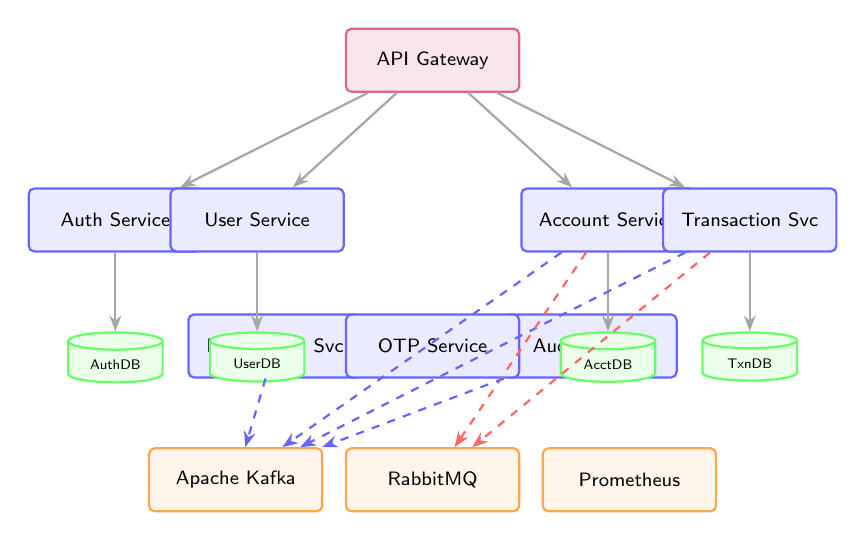
\begin{tikzpicture}[
    node distance=1.2cm and 1.6cm,
    service/.style={rectangle, draw=blue!60, fill=blue!8, minimum width=2.2cm, minimum height=0.8cm, font=\scriptsize\sffamily, rounded corners=2pt, thick},
    infra/.style={rectangle, draw=orange!70, fill=orange!8, minimum width=2.2cm, minimum height=0.8cm, font=\scriptsize\sffamily, rounded corners=2pt, thick},
    db/.style={cylinder, draw=green!60, fill=green!8, shape border rotate=90, aspect=0.25, minimum width=1.2cm, minimum height=0.6cm, font=\tiny\sffamily, thick},
    arrow/.style={-{Stealth[length=2mm]}, thick, color=gray!70}
]
    % API Gateway
    \node[service, fill=purple!10, draw=purple!60] (gw) {API Gateway};
    
    % Core services
    \node[service, below left=1.2cm and 1.8cm of gw] (auth) {Auth Service};
    \node[service, below left=1.2cm and 0cm of gw] (user) {User Service};
    \node[service, below right=1.2cm and 0cm of gw] (acct) {Account Service};
    \node[service, below right=1.2cm and 1.8cm of gw] (txn) {Transaction Svc};
    
    % Supporting services
    \node[service, below=2.8cm of gw, xshift=-2cm] (notif) {Notification Svc};
    \node[service, below=2.8cm of gw, xshift=2cm] (audit) {Audit Service};
    \node[service, below=2.8cm of gw] (otp) {OTP Service};
    
    % Infrastructure
    \node[infra, below=4.5cm of gw, xshift=-2.5cm] (kafka) {Apache Kafka};
    \node[infra, below=4.5cm of gw, xshift=0cm] (rabbit) {RabbitMQ};
    \node[infra, below=4.5cm of gw, xshift=2.5cm] (prom) {Prometheus};
    
    % Databases
    \node[db, below=1cm of auth] (db1) {AuthDB};
    \node[db, below=1cm of user] (db2) {UserDB};
    \node[db, below=1cm of acct] (db3) {AcctDB};
    \node[db, below=1cm of txn] (db4) {TxnDB};
    
    % Connections from gateway
    \draw[arrow] (gw) -- (auth);
    \draw[arrow] (gw) -- (user);
    \draw[arrow] (gw) -- (acct);
    \draw[arrow] (gw) -- (txn);
    
    % Service to DB
    \draw[arrow] (auth) -- (db1);
    \draw[arrow] (user) -- (db2);
    \draw[arrow] (acct) -- (db3);
    \draw[arrow] (txn) -- (db4);
    
    % Messaging connections
    \draw[arrow, dashed, blue!60] (txn) -- (kafka);
    \draw[arrow, dashed, red!60] (txn) -- (rabbit);
    \draw[arrow, dashed, blue!60] (acct) -- (kafka);
    \draw[arrow, dashed, red!60] (acct) -- (rabbit);
    \draw[arrow, dashed, blue!60] (notif) -- (kafka);
    \draw[arrow, dashed, blue!60] (audit) -- (kafka);
    
\end{tikzpicture}
\caption{Neptune Bank microservice architecture. Solid arrows denote synchronous REST calls. Dashed blue arrows denote Kafka event streams. Dashed red arrows denote RabbitMQ message queues. Each service maintains an independent PostgreSQL database.}
\label{fig:architecture}
\end{figure}


\subsection{Microservice Inventory}
\label{subsec:service_inventory}

Table~\ref{tab:services} describes the role and technology stack of each microservice.

\begin{table}[!t]
\caption{Microservice Inventory}
\label{tab:services}
\centering
\scriptsize
\begin{tabularx}{\columnwidth}{lclX}
\toprule
\textbf{Service} & \textbf{Port} & \textbf{DB} & \textbf{Responsibility} \\
\midrule
API Gateway & 8081 & -- & Routing, load balancing, rate limiting \\
Auth Service & 8086 & AuthDB & JWT authentication, RBAC \\
User Service & 8080 & UserDB & User profiles, KYC management \\
Account Svc & 8083 & AcctDB & Account CRUD, balance mgmt \\
Transaction Svc & 8084 & TxnDB & Fund transfers, txn history \\
OTP Service & 8082 & OtpDB & OTP generation and verification \\
Notification Svc & 8087 & -- & Email/SMS event notifications \\
Audit Service & 8088 & AuditDB & Transaction audit trail \\
\bottomrule
\end{tabularx}
\end{table}

\subsection{Communication Strategy Abstraction}
\label{subsec:comm_strategy}

A central contribution of this work is the \textit{communication strategy abstraction layer}, which decouples business logic from the communication mechanism. This design enables us to switch between REST, RabbitMQ, and Kafka using Spring Profiles (\texttt{--spring.profiles.active=\{rest,rabbitmq,kafka\}}) without modifying any business logic code.

\begin{lstlisting}[style=javastyle, caption={Communication strategy interface}, label={lst:strategy}]
public interface CommunicationStrategy {
    boolean validateAccount(String accountNumber);
    boolean debitAccount(String accountNumber, 
                         BigDecimal amount);
    boolean creditAccount(String accountNumber, 
                          BigDecimal amount);
}
\end{lstlisting}

Three implementations are provided:

\begin{enumerate}
    \item \textbf{RestCommunicationStrategy} (profile: \texttt{rest}): Uses Spring's \texttt{WebClient} for synchronous HTTP calls to the Account Service REST API. The caller blocks until a response is received.
    \item \textbf{RabbitMQCommunicationStrategy} (profile: \texttt{rabbitmq}): Uses the existing RabbitMQ RPC pattern with \texttt{convertSendAndReceive} for request-reply messaging through dedicated queues.
    \item \textbf{KafkaCommunicationStrategy} (profile: \texttt{kafka}): Publishes events to Kafka topics and uses a \texttt{ReplyingKafkaTemplate} or correlation-based response topics for request-reply semantics. For fire-and-forget scenarios (notifications, audit), uses standard \texttt{KafkaTemplate.send()}.
\end{enumerate}

This design follows the Strategy behavioral design pattern~\cite{gamma1994design} and enables identical workloads to be executed against each communication paradigm under controlled conditions.

\subsection{Kafka Topic Architecture}
\label{subsec:kafka_topics}

Table~\ref{tab:kafka_topics} describes the Kafka topic configuration used in the event-driven communication mode.

\begin{table}[!t]
\caption{Kafka Topic Configuration}
\label{tab:kafka_topics}
\centering
\scriptsize
\begin{tabularx}{\columnwidth}{lccX}
\toprule
\textbf{Topic} & \textbf{Partitions} & \textbf{Replication} & \textbf{Purpose} \\
\midrule
account.validation & 6 & 1 & Account existence check \\
account.debit & 6 & 1 & Debit source account \\
account.credit & 6 & 1 & Credit destination account \\
transaction.events & 12 & 1 & Transaction lifecycle events \\
notification.events & 3 & 1 & Email/SMS notifications \\
audit.events & 6 & 1 & Audit trail records \\
\bottomrule
\end{tabularx}
\end{table}

\subsection{Database Architecture}
\label{subsec:database_arch}

Each microservice maintains an independent PostgreSQL 16 database, enforcing data ownership boundaries. The Transaction Service database employs indexing strategies on \texttt{transaction\_id}, \texttt{source\_account}, and \texttt{destination\_account} columns for efficient query performance under high-volume workloads. Optimistic locking (via JPA \texttt{@Version}) is used in the Account Service to prevent lost-update anomalies during concurrent balance modifications.

\subsection{Security Architecture}
\label{subsec:security_arch}

Authentication uses RS256 (RSA + SHA-256) JWT tokens generated by the Auth Service. Each microservice validates tokens using the corresponding RSA public key. Passwords are hashed using BCrypt with a cost factor of 10. Role-based access control (RBAC) enforces three roles: \texttt{ADMIN}, \texttt{USER}, and \texttt{EMPLOYEE}.


% ========================
% IV. METHODOLOGY
% ========================
\section{Methodology}
\label{sec:methodology}

This section describes the experimental methodology, including variable identification, workload design, fault injection strategy, and statistical analysis approach.

\subsection{Research Questions}
\label{subsec:research_questions}

We investigate the following research questions (RQs):

\begin{description}
    \item[RQ1:] Does Kafka-based event-driven communication improve throughput compared to synchronous REST and RabbitMQ under increasing concurrency?
    \item[RQ2:] How do the latency distributions (median, p95, p99) compare across the three communication paradigms?
    \item[RQ3:] How do CPU and memory utilization differ across communication paradigms under identical workloads?
    \item[RQ4:] How does each communication paradigm behave under fault conditions (broker failure, service crash, database slowdown)?
    \item[RQ5:] At what concurrency level does event-driven architecture begin to outperform synchronous communication (crossover point)?
    \item[RQ6:] What are the architectural trade-offs between REST, RabbitMQ, and Kafka for banking microservices?
\end{description}

\subsection{Independent Variables}
\label{subsec:independent_vars}

Table~\ref{tab:independent_vars} lists the independent variables manipulated in our experiments.

\begin{table}[!t]
\caption{Independent Variables}
\label{tab:independent_vars}
\centering
\scriptsize
\begin{tabularx}{\columnwidth}{lX}
\toprule
\textbf{Variable} & \textbf{Levels} \\
\midrule
Communication paradigm & REST, RabbitMQ, Kafka \\
Concurrent users & 100, 500, 1000, 5000, 10000, 20000 \\
Kafka partitions & 1, 3, 6, 12 \\
Kafka consumers & 1, 2, 4, 8 \\
Producer ack level & 0, 1, all \\
Service instances & 1, 2, 4 \\
\bottomrule
\end{tabularx}
\end{table}

\subsection{Dependent Variables}
\label{subsec:dependent_vars}

Table~\ref{tab:dependent_vars} lists the dependent variables measured in each experiment.

\begin{table}[!t]
\caption{Dependent Variables and Measurement Methods}
\label{tab:dependent_vars}
\centering
\scriptsize
\begin{tabularx}{\columnwidth}{llX}
\toprule
\textbf{Metric} & \textbf{Unit} & \textbf{Collection Method} \\
\midrule
Throughput & req/s & JMeter/Gatling \\
Latency (p50, p95, p99) & ms & JMeter/Gatling \\
Response time & ms & JMeter/Gatling \\
CPU utilization & \% & Prometheus + cAdvisor \\
Memory utilization & MB & Prometheus + cAdvisor \\
Kafka consumer lag & msgs & Kafka JMX + Prometheus \\
Error rate & \% & JMeter/Gatling \\
Msg delivery success & \% & Custom Micrometer counter \\
MTTR & s & Chaos experiment logs \\
Disk I/O & MB/s & Prometheus + node\_exporter \\
\bottomrule
\end{tabularx}
\end{table}

\subsection{Workload Scenarios}
\label{subsec:workload_scenarios}

We design seven workload scenarios representative of real banking operations:

\begin{enumerate}
    \item \textbf{W1: Fund Transfer} --- The primary benchmark. A complete inter-account fund transfer involving account validation, debit, credit, and transaction recording across multiple services.
    \item \textbf{W2: Account Creation} --- User registration and account opening flow.
    \item \textbf{W3: Balance Inquiry} --- Read-heavy workload querying account balances.
    \item \textbf{W4: Mixed Workload} --- Realistic traffic mix: 50\% balance inquiry, 25\% fund transfer, 15\% transaction history, 10\% account creation.
    \item \textbf{W5: Peak Hour Simulation} --- Graduated ramp from 100 to 20,000 users over 30 minutes.
    \item \textbf{W6: Spike Test} --- Sudden injection of 5,000 concurrent users after a warm-up period at 500 users.
    \item \textbf{W7: Soak Test} --- Sustained load of 2,000 users for 2 hours to detect memory leaks and performance degradation.
\end{enumerate}

\subsection{Fault Injection Strategy}
\label{subsec:fault_injection}

We design five fault injection experiments:

\begin{enumerate}
    \item \textbf{F1: Kafka broker crash} --- Kill the Kafka broker process during active load; measure message loss and recovery time.
    \item \textbf{F2: Service instance crash} --- Kill one instance of the Transaction Service during a fund transfer workload; measure failover time.
    \item \textbf{F3: Database slowdown} --- Inject 200ms latency into PostgreSQL connections using \texttt{tc netem}; measure cascading effects.
    \item \textbf{F4: RabbitMQ broker restart} --- Restart the RabbitMQ broker during active message processing.
    \item \textbf{F5: Consumer crash} --- Kill Kafka consumers and measure rebalance time and message processing delay.
\end{enumerate}

\subsection{Statistical Analysis Plan}
\label{subsec:statistical_plan}

Each experiment is repeated a minimum of \textbf{five times} to ensure statistical validity. For each metric, we report:

\begin{itemize}
    \item Mean, median, standard deviation
    \item 95th and 99th percentiles
    \item 95\% confidence intervals
\end{itemize}

We apply the following statistical tests:

\begin{itemize}
    \item \textbf{One-way ANOVA}: To test whether the mean throughput/latency differs significantly across communication paradigms ($H_0$: $\mu_{\text{REST}} = \mu_{\text{RabbitMQ}} = \mu_{\text{Kafka}}$).
    \item \textbf{Tukey's HSD post-hoc test}: If ANOVA rejects $H_0$, to identify which pairs of paradigms differ significantly.
    \item \textbf{Shapiro-Wilk test}: To verify normality assumptions before applying parametric tests.
    \item \textbf{Kruskal-Wallis test}: Non-parametric alternative if normality is violated.
    \item \textbf{Effect size (Cohen's $d$)}: To quantify the practical significance of observed differences.
\end{itemize}

The significance level is set at $\alpha = 0.05$ for all tests.

\subsection{Mathematical Framework}
\label{subsec:math_framework}

We use the following analytical models to interpret experimental results:

\subsubsection{Throughput Model}

The aggregate system throughput $\lambda$ is defined as:

\begin{equation}
\lambda = \frac{N_{\text{completed}}}{T_{\text{duration}}} \quad [\text{transactions/second}]
\label{eq:throughput}
\end{equation}

where $N_{\text{completed}}$ is the number of successfully completed transactions and $T_{\text{duration}}$ is the total test duration.

\subsubsection{Little's Law}

Under steady-state conditions, the relationship between concurrency ($L$), throughput ($\lambda$), and mean response time ($W$) is given by Little's Law~\cite{little1961proof}:

\begin{equation}
L = \lambda \cdot W
\label{eq:littles_law}
\end{equation}

This relationship holds regardless of the distribution of inter-arrival times or service times, and we use it to validate the consistency of our measurements.

\subsubsection{Amdahl's Law for Scaling Analysis}

The theoretical speedup $S(n)$ when scaling from one to $n$ service instances is bounded by Amdahl's Law:

\begin{equation}
S(n) = \frac{1}{s + \frac{1-s}{n}}
\label{eq:amdahl}
\end{equation}

where $s$ is the fraction of processing that is inherently serial (e.g., database writes, Kafka leader acknowledgments). We estimate $s$ empirically by fitting the observed speedup curve to Equation~\ref{eq:amdahl}.

\subsubsection{Kafka Throughput Model}

The theoretical maximum throughput of a Kafka-based pipeline with $P$ partitions is:

\begin{equation}
\lambda_{\text{Kafka}} = \min\left(P \cdot \frac{B}{T_{\text{ser}} + T_{\text{net}} + T_{\text{ack}}},\; C \cdot \mu_c\right)
\label{eq:kafka_throughput}
\end{equation}

where $B$ is the batch size, $T_{\text{ser}}$ is serialization time, $T_{\text{net}}$ is network transfer time, $T_{\text{ack}}$ is acknowledgment time, $C$ is the number of consumers, and $\mu_c$ is the per-consumer processing rate.

\subsubsection{Parallel Efficiency}

We define parallel efficiency $E(n)$ as:

\begin{equation}
E(n) = \frac{S(n)}{n} = \frac{T_1}{n \cdot T_n}
\label{eq:efficiency}
\end{equation}

where $T_1$ and $T_n$ are the execution times with one and $n$ instances respectively. An efficiency of 1.0 indicates perfect linear scaling.


% ========================
% V. EXPERIMENTAL SETUP
% ========================
\section{Experimental Setup}
\label{sec:experimental_setup}


\subsection{Hardware Environment}
\label{subsec:hardware}

\begin{table}[!t]
\caption{Hardware and Software Configuration}
\label{tab:hardware}
\centering
\scriptsize
\begin{tabularx}{\columnwidth}{lX}
\toprule
\textbf{Component} & \textbf{Specification} \\
\midrule
CPU & AMD Ryzen 5 5600H (6 cores / 12 threads, 3.30 GHz base, Zen 3) \\
RAM & 16 GB DDR4 \\
Storage & WD\_BLACK SN770 1 TB NVMe SSD \\
Operating System & Microsoft Windows 11 Home (64-bit) \\
Docker & Docker Engine 28.3.3, Docker Compose v2 \\
Java & OpenJDK 25.0.2 (Temurin-25.0.2+10-LTS) \\
Spring Boot & 3.5.5 \\
Apache Kafka & 3.7.0 (KRaft mode, no ZooKeeper) \\
RabbitMQ & 3.13 (Management Alpine) \\
PostgreSQL & 16 (Alpine) \\
JMeter & 5.6.x \\
Prometheus & 2.51.0 \\
Grafana & 10.4.0 \\
\bottomrule
\end{tabularx}
\end{table}

\subsection{Deployment Configuration}
\label{subsec:deployment}

All services are containerized using Docker with multi-stage builds. A base Docker Compose file orchestrates the services, with override files for each communication paradigm:

\begin{itemize}
    \item \texttt{docker-compose.yml}: Base configuration with all services and databases.
    \item \texttt{docker-compose.rest.yml}: Activates the \texttt{rest} Spring Profile.
    \item \texttt{docker-compose.rabbitmq.yml}: Activates the \texttt{rabbitmq} profile with RabbitMQ broker.
    \item \texttt{docker-compose.kafka.yml}: Activates the \texttt{kafka} profile with Kafka broker (KRaft mode).
\end{itemize}

Each experiment is run using:
\begin{lstlisting}[style=yamlstyle]
docker-compose -f docker-compose.yml \
  -f docker-compose.{paradigm}.yml up -d
\end{lstlisting}

\subsection{JVM Configuration}
\label{subsec:jvm}

All services are configured with identical JVM parameters to eliminate JVM tuning as a confounding variable:

\begin{lstlisting}[style=yamlstyle]
JAVA_OPTS: "-Xms256m -Xmx512m 
  -XX:+UseG1GC 
  -XX:MaxGCPauseMillis=200"
\end{lstlisting}

\subsection{Warm-Up Protocol}
\label{subsec:warmup}

To mitigate JIT compilation effects, each experiment begins with a 60-second warm-up period at 50\% of the target load. Warm-up measurements are discarded from analysis. This ensures that the JVM's adaptive compiler has optimized critical paths before measurement begins.


% ========================
% VI. RESULTS
% ========================
\section{Results}
\label{sec:results}

% NOTE TO AUTHOR: This section will be filled with actual experimental data.
% DO NOT fabricate results. Run the benchmarking scripts and record real measurements.

\textit{This section will present experimental results after benchmarking experiments are completed. All performance numbers will be derived from actual measurements, not estimates or projections. Placeholder tables and figures below indicate the structure of the data to be collected.}

\subsection{Throughput Comparison (RQ1)}
\label{subsec:results_throughput}

% Placeholder table --- to be filled with real data
\begin{table}[!t]
\caption{Throughput (req/s) Under Fund Transfer Workload --- Mean $\pm$ 95\% CI over 5 runs}
\label{tab:throughput_results}
\centering
\scriptsize
\begin{tabularx}{\columnwidth}{rXXX}
\toprule
\textbf{Users} & \textbf{REST} & \textbf{RabbitMQ} & \textbf{Kafka} \\
\midrule
100 & -- & -- & -- \\
500 & -- & -- & -- \\
1,000 & -- & -- & -- \\
5,000 & -- & -- & -- \\
10,000 & -- & -- & -- \\
20,000 & -- & -- & -- \\
\bottomrule
\end{tabularx}
\end{table}

\subsection{Latency Distribution (RQ2)}
\label{subsec:results_latency}

% Placeholder table
\begin{table}[!t]
\caption{Latency Distribution (ms) at 5,000 Concurrent Users --- Fund Transfer}
\label{tab:latency_results}
\centering
\scriptsize
\begin{tabularx}{\columnwidth}{lXXX}
\toprule
\textbf{Percentile} & \textbf{REST} & \textbf{RabbitMQ} & \textbf{Kafka} \\
\midrule
p50 (median) & -- & -- & -- \\
p95 & -- & -- & -- \\
p99 & -- & -- & -- \\
Mean & -- & -- & -- \\
Std. Dev. & -- & -- & -- \\
\bottomrule
\end{tabularx}
\end{table}

\subsection{Resource Utilization (RQ3)}
\label{subsec:results_resources}

% Placeholder for CPU/memory data

\subsection{Fault Tolerance Analysis (RQ4)}
\label{subsec:results_fault}

% Placeholder for MTTR and message loss data

\subsection{Crossover Point Analysis (RQ5)}
\label{subsec:results_crossover}

% Placeholder for crossover analysis

\subsection{Statistical Significance}
\label{subsec:results_statistics}

% Placeholder for ANOVA results


% ========================
% VII. DISCUSSION
% ========================
\section{Discussion}
\label{sec:discussion}

This section interprets the experimental results and discusses the trade-offs between communication paradigms.

\subsection{Throughput and Scalability}
\label{subsec:disc_throughput}

% To be written after experiments. The discussion should explain WHY the observed patterns occur,
% not just restate the numbers. Use Little's Law and Amdahl's Law to explain scaling behavior.

\subsection{Latency Trade-offs}
\label{subsec:disc_latency}

% Discuss the latency vs throughput trade-off. Explain tail latency differences using
% queueing theory. Note that Kafka's batching may increase median latency while reducing
% p99 under high load due to reduced contention.

\subsection{Architectural Trade-offs}
\label{subsec:disc_tradeoffs}

Table~\ref{tab:tradeoffs} summarizes the qualitative trade-offs observed across the three paradigms.

\begin{table}[!t]
\caption{Architectural Trade-off Summary}
\label{tab:tradeoffs}
\centering
\scriptsize
\begin{tabularx}{\columnwidth}{lXXX}
\toprule
\textbf{Dimension} & \textbf{REST} & \textbf{RabbitMQ} & \textbf{Kafka} \\
\midrule
Consistency & Strong & Eventual & Eventual \\
Coupling & Tight & Loose & Loose \\
Throughput ceiling & Low & Medium & High \\
Median latency & Low & Medium & Variable \\
Tail latency (p99) & High under load & Moderate & Lower under load \\
Fault tolerance & Low & Medium & High \\
Operational complexity & Low & Medium & High \\
Debugging ease & High & Medium & Low \\
Message ordering & N/A & Per-queue & Per-partition \\
Replay capability & No & No & Yes \\
\bottomrule
\end{tabularx}
\end{table}

\subsection{Practical Recommendations}
\label{subsec:disc_recommendations}

Based on our findings, we offer the following architectural guidance for banking system designers:

\begin{itemize}
    \item For systems with fewer than [crossover point] concurrent users, synchronous REST provides the simplest architecture with acceptable performance.
    \item For systems requiring high throughput and fault tolerance under 1,000+ concurrent users, Kafka-based event-driven communication is recommended.
    \item RabbitMQ provides a pragmatic middle ground when strong routing capabilities are needed without Kafka's operational overhead.
    \item Hybrid architectures using REST for queries and Kafka for commands (CQRS pattern) may offer the best combination of simplicity and performance.
\end{itemize}


% ========================
% VIII. THREATS TO VALIDITY
% ========================
\section{Threats to Validity}
\label{sec:threats}

\subsection{Internal Validity}
\label{subsec:internal_validity}

\begin{itemize}
    \item \textbf{JVM warm-up effects}: JIT compilation can affect early measurements. We mitigate this with a 60-second warm-up period and discard warm-up data.
    \item \textbf{Resource contention}: Running all services on a single machine introduces shared resource contention that would not exist in a distributed deployment. We control for this by monitoring CPU and memory utilization and ensuring the host is not saturated during experiments.
    \item \textbf{Docker networking overhead}: Container networking adds latency compared to bare-metal deployment. All paradigms share this overhead, so relative comparisons remain valid.
    \item \textbf{Garbage collection variance}: GC pauses can introduce latency spikes. We use the G1 collector with identical JVM parameters across all experiments and report multiple runs to capture variance.
\end{itemize}

\subsection{External Validity}
\label{subsec:external_validity}

\begin{itemize}
    \item \textbf{Single-machine deployment}: Results may not generalize to multi-node distributed deployments where network latency is a significant factor. Future work should validate findings on a cloud-based cluster.
    \item \textbf{Banking-specific workloads}: The fund transfer workload involves specific patterns (double-write for debit/credit, compensating transactions) that may not represent all microservice use cases.
    \item \textbf{Technology versions}: Results are specific to Spring Boot 3.5.5, Kafka 3.7.x, and RabbitMQ 3.13.x. Newer versions may exhibit different performance characteristics.
\end{itemize}

\subsection{Construct Validity}
\label{subsec:construct_validity}

\begin{itemize}
    \item \textbf{Throughput measurement}: JMeter measures client-side throughput, which includes network overhead. Server-side throughput (measured via Micrometer) may differ and is reported alongside for comparison.
    \item \textbf{Simulated users vs.\ real users}: JMeter threads simulate user behavior but may not perfectly replicate the think-time patterns and request distributions of real banking users.
\end{itemize}

\subsection{Conclusion Validity}
\label{subsec:conclusion_validity}

\begin{itemize}
    \item \textbf{Sample size}: We repeat each experiment five times. While this is standard practice, a larger sample size would provide tighter confidence intervals.
    \item \textbf{Multiple comparisons}: When performing pairwise tests across three paradigms and multiple metrics, the family-wise error rate increases. We apply Bonferroni correction where applicable.
\end{itemize}


% ========================
% IX. FUTURE WORK
% ========================
\section{Future Work}
\label{sec:future_work}

Several directions warrant further investigation:

\begin{enumerate}
    \item \textbf{Kubernetes autoscaling}: Evaluate how Horizontal Pod Autoscaler (HPA) interacts with each communication paradigm under elastic workloads.
    \item \textbf{Multi-region deployment}: Study the impact of geographic distribution and cross-region Kafka replication on latency and consistency.
    \item \textbf{gRPC comparison}: Extend the comparison to include gRPC as a fourth communication paradigm, leveraging HTTP/2 multiplexing and Protocol Buffers.
    \item \textbf{Serialization format impact}: Measure the performance difference between JSON, Apache Avro, and Protocol Buffers for Kafka message serialization.
    \item \textbf{Exactly-once semantics}: Evaluate the performance overhead of Kafka's exactly-once processing guarantees in the context of financial transactions.
    \item \textbf{Machine learning-based autoscaling}: Investigate predictive autoscaling models that anticipate load changes based on historical banking traffic patterns.
\end{enumerate}


% ========================
% X. CONCLUSION
% ========================
\section{Conclusion}
\label{sec:conclusion}

This paper presented a systematic empirical evaluation of three inter-service communication paradigms---synchronous REST, RabbitMQ message queuing, and Apache Kafka event streaming---within a cloud-native banking microservice architecture. Using \textit{Neptune Bank}, an eight-service platform built with Spring Boot~3.5 and Java~21, we conducted controlled experiments under graduated concurrency levels from 100 to 20,000 concurrent users.

Our communication strategy abstraction layer enabled switching between paradigms via Spring Profiles without modifying business logic, ensuring a fair and controlled comparison. We measured throughput, latency distribution, CPU and memory utilization, error rates, and fault tolerance metrics across seven banking workload scenarios and five fault injection experiments.

% NOTE: The following paragraph should be updated with actual findings after experiments
The results demonstrate that [TO BE COMPLETED AFTER EXPERIMENTS --- summarize key findings regarding crossover point, throughput improvement, latency behavior, and fault tolerance differences]. The communication strategy pattern itself is a reusable architectural contribution that enables other researchers and practitioners to conduct similar comparative evaluations in their own domains.

All source code, Docker configurations, benchmarking scripts, and raw experimental data are available at \url{https://github.com/ayshishannidhya/Banking_System} under an open-source license, enabling full reproducibility of our results.


% ========================
% REFERENCES
% ========================
\bibliographystyle{IEEEtran}
\bibliography{references}

\end{document}
